\documentclass[]{article}
\usepackage{lmodern}
\usepackage{amssymb,amsmath}
\usepackage{ifxetex,ifluatex}
\usepackage{fixltx2e} % provides \textsubscript
\ifnum 0\ifxetex 1\fi\ifluatex 1\fi=0 % if pdftex
  \usepackage[T1]{fontenc}
  \usepackage[utf8]{inputenc}
\else % if luatex or xelatex
  \ifxetex
    \usepackage{mathspec}
  \else
    \usepackage{fontspec}
  \fi
  \defaultfontfeatures{Ligatures=TeX,Scale=MatchLowercase}
\fi
% use upquote if available, for straight quotes in verbatim environments
\IfFileExists{upquote.sty}{\usepackage{upquote}}{}
% use microtype if available
\IfFileExists{microtype.sty}{%
\usepackage{microtype}
\UseMicrotypeSet[protrusion]{basicmath} % disable protrusion for tt fonts
}{}
\usepackage[margin=1in]{geometry}
\usepackage{hyperref}
\hypersetup{unicode=true,
            pdftitle={Statistical Report},
            pdfauthor={Committee},
            pdfborder={0 0 0},
            breaklinks=true}
\urlstyle{same}  % don't use monospace font for urls
\usepackage{graphicx,grffile}
\makeatletter
\def\maxwidth{\ifdim\Gin@nat@width>\linewidth\linewidth\else\Gin@nat@width\fi}
\def\maxheight{\ifdim\Gin@nat@height>\textheight\textheight\else\Gin@nat@height\fi}
\makeatother
% Scale images if necessary, so that they will not overflow the page
% margins by default, and it is still possible to overwrite the defaults
% using explicit options in \includegraphics[width, height, ...]{}
\setkeys{Gin}{width=\maxwidth,height=\maxheight,keepaspectratio}
\IfFileExists{parskip.sty}{%
\usepackage{parskip}
}{% else
\setlength{\parindent}{0pt}
\setlength{\parskip}{6pt plus 2pt minus 1pt}
}
\setlength{\emergencystretch}{3em}  % prevent overfull lines
\providecommand{\tightlist}{%
  \setlength{\itemsep}{0pt}\setlength{\parskip}{0pt}}
\setcounter{secnumdepth}{5}
% Redefines (sub)paragraphs to behave more like sections
\ifx\paragraph\undefined\else
\let\oldparagraph\paragraph
\renewcommand{\paragraph}[1]{\oldparagraph{#1}\mbox{}}
\fi
\ifx\subparagraph\undefined\else
\let\oldsubparagraph\subparagraph
\renewcommand{\subparagraph}[1]{\oldsubparagraph{#1}\mbox{}}
\fi

%%% Use protect on footnotes to avoid problems with footnotes in titles
\let\rmarkdownfootnote\footnote%
\def\footnote{\protect\rmarkdownfootnote}

%%% Change title format to be more compact
\usepackage{titling}

% Create subtitle command for use in maketitle
\providecommand{\subtitle}[1]{
  \posttitle{
    \begin{center}\large#1\end{center}
    }
}

\setlength{\droptitle}{-2em}

  \title{Statistical Report}
    \pretitle{\vspace{\droptitle}\centering\huge}
  \posttitle{\par}
    \author{Committee}
    \preauthor{\centering\large\emph}
  \postauthor{\par}
      \predate{\centering\large\emph}
  \postdate{\par}
    \date{November 4, 2018}

\usepackage{float}
\usepackage{longtable}

\begin{document}
\maketitle

{
\setcounter{tocdepth}{2}
\tableofcontents
}
\begin{center}\rule{0.5\linewidth}{\linethickness}\end{center}

\hypertarget{the-human-freedom-index}{%
\subsection{The Human Freedom Index}\label{the-human-freedom-index}}

``The Human Freedom Index presents the state of human freedom in the
world based on a broad measure that encompasses personal, civil, and
economic freedom.''

The report is co-published by the Cato Institute, the Fraser Institute,
and the Liberales Institut at the Friedrich Naumann Foundation for
Freedom. For more details on the Human Freedom Index Project, see
\url{https://www.cato.org/human-freedom-index-new}.

\hypertarget{project-topic}{%
\subsection{Project Topic}\label{project-topic}}

The Human Index freedom is constructed of 162 counties that combines
economic freedom measurements with personal freedom measurements. The
index aims to understand the degree of freedom people are able to enjoy
classic civil liberties from the countries that were surveyed. We will
investigate the correlations between personal and economic freedom to
see if one can be a predictor for the other, and specifically examine
the subcategories of the two indeces.

\hypertarget{personal-freedom}{%
\subsection{Personal Freedom}\label{personal-freedom}}

\begin{itemize}
\tightlist
\item
  Rule of Law (rol)
\item
  Security and Safety (safety)
\item
  Movement (movement)
\item
  Religion (religion)
\item
  Association, Assembly, and Civil Society (assembly)
\item
  Expression and Information (expression)
\item
  Identity and Relationships (relationships)
\end{itemize}

\hypertarget{economic-freedom}{%
\subsection{Economic Freedom}\label{economic-freedom}}

\begin{itemize}
\tightlist
\item
  Size of Government (govsize)
\item
  Legal System and Property Rights (legalsystems)
\item
  Access to Sound Money (money)
\item
  Freedom to Trade Internationally (trade)
\item
  Regulation of Credit, Labor, and Business (regulation)
\end{itemize}

\hypertarget{summary-of-personal-freedom-index}{%
\subsection{Summary of Personal Freedom
Index}\label{summary-of-personal-freedom-index}}

The personal freedom sub-index is comprised of 34 numerical variables
divided into six categories. The indicators are rated on a sale of 1 to
10, with 10 representing the most freedom.

\begin{verbatim}
##    Min. 1st Qu.  Median    Mean 3rd Qu.    Max. 
##   2.167   6.025   6.932   6.985   8.142   9.399
\end{verbatim}

\hypertarget{summary-of-economic-freedom-index}{%
\subsection{Summary of Economic Freedom
Index}\label{summary-of-economic-freedom-index}}

The economic freedom sub-index is comprised of 42 numerical variables
divided into five categories. The indicators are rated on a sale of 1 to
10, with 10 representing the most freedom.

\begin{verbatim}
##    Min. 1st Qu.  Median    Mean 3rd Qu.    Max. 
##   2.880   6.260   6.905   6.795   7.468   8.970
\end{verbatim}

\hypertarget{economic-freedom-vs.personal-freedom}{%
\subsection{Economic Freedom vs.~Personal
Freedom}\label{economic-freedom-vs.personal-freedom}}

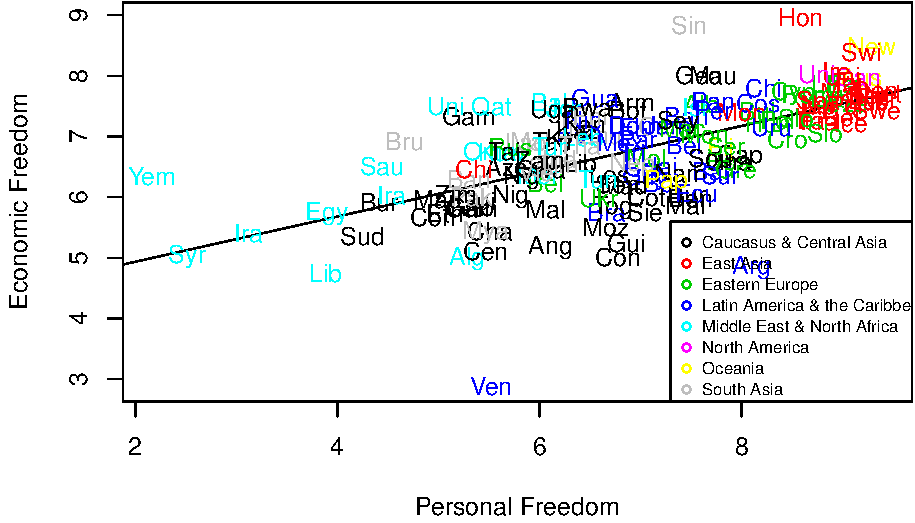
\includegraphics{final_presentation_files/figure-latex/fig1-1.pdf} There
is a clear positive correlation between personal and economic freedom,
with a correlation of 0.6271777.

\hypertarget{economic-freedom-vs.rule-of-law}{%
\subsection{Economic Freedom vs.~Rule of
Law}\label{economic-freedom-vs.rule-of-law}}

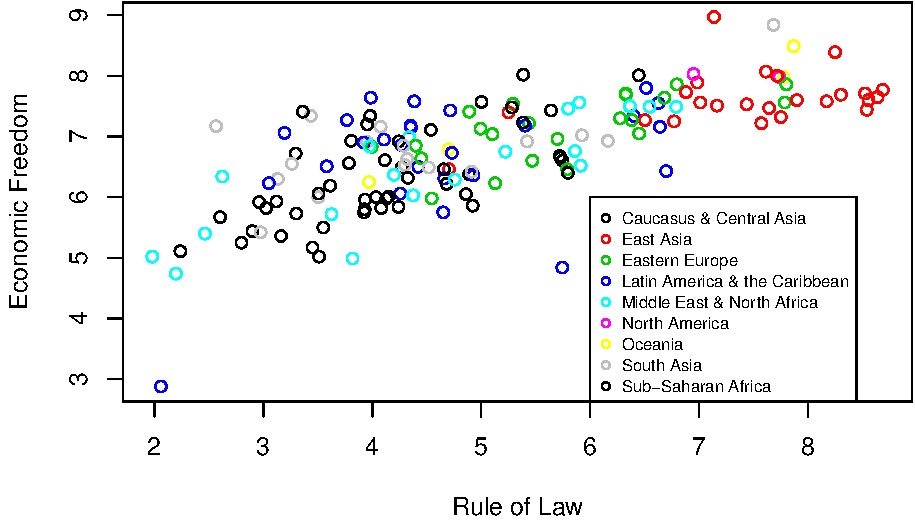
\includegraphics{final_presentation_files/figure-latex/unnamed-chunk-3-1.pdf}

\hypertarget{economic-freedom-vs.security-and-safety}{%
\subsection{Economic Freedom vs.~Security and
Safety}\label{economic-freedom-vs.security-and-safety}}

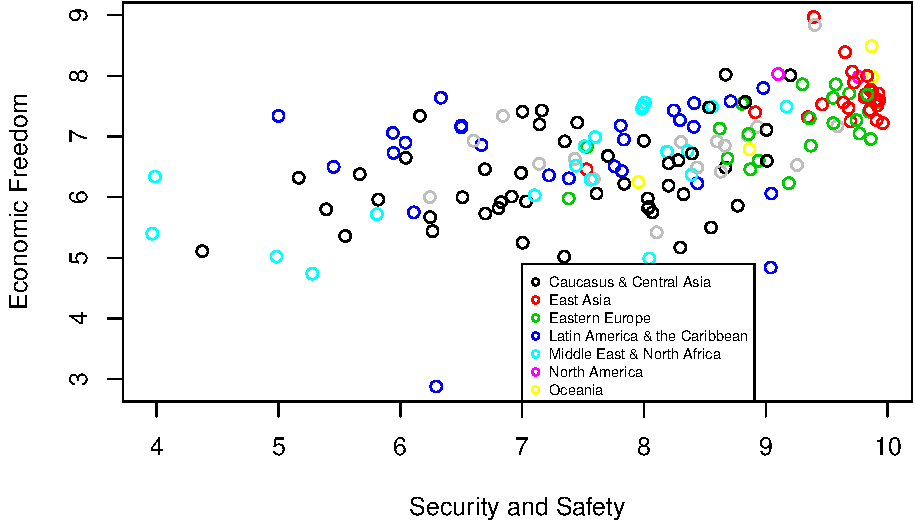
\includegraphics{final_presentation_files/figure-latex/unnamed-chunk-4-1.pdf}

\hypertarget{economic-freedom-vs.movement}{%
\subsection{Economic Freedom
vs.~Movement}\label{economic-freedom-vs.movement}}

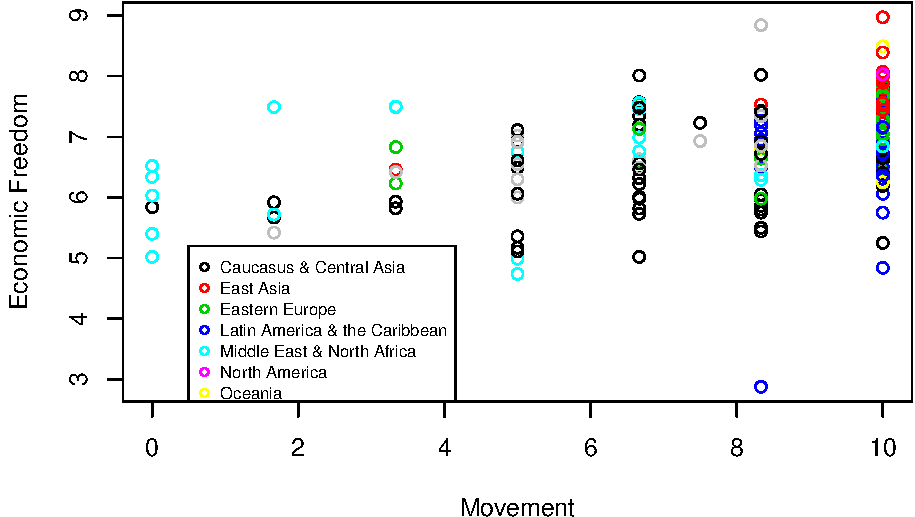
\includegraphics{final_presentation_files/figure-latex/unnamed-chunk-5-1.pdf}

\hypertarget{economic-freedom-vs.religion}{%
\subsection{Economic Freedom
vs.~Religion}\label{economic-freedom-vs.religion}}

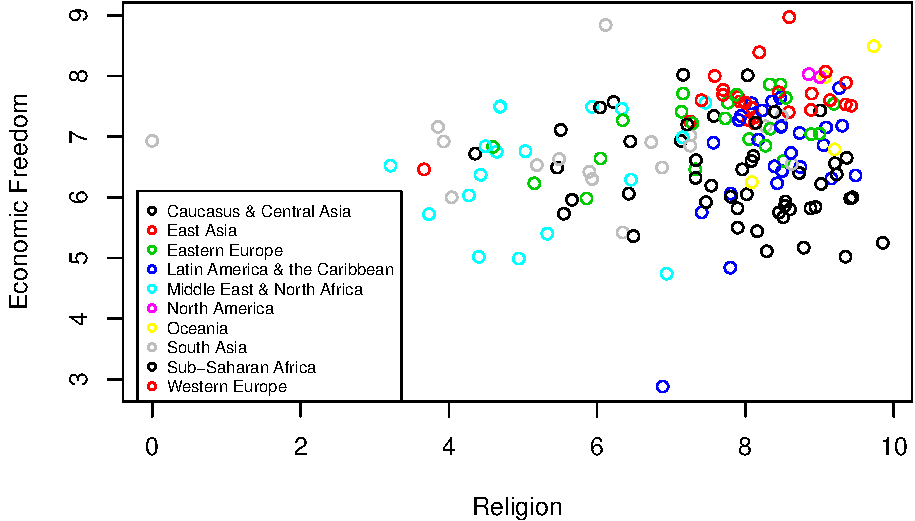
\includegraphics{final_presentation_files/figure-latex/unnamed-chunk-6-1.pdf}

\hypertarget{economic-freedom-vs.association-assembly-and-civil-society}{%
\subsection{Economic Freedom vs.~Association, Assembly, and Civil
Society}\label{economic-freedom-vs.association-assembly-and-civil-society}}

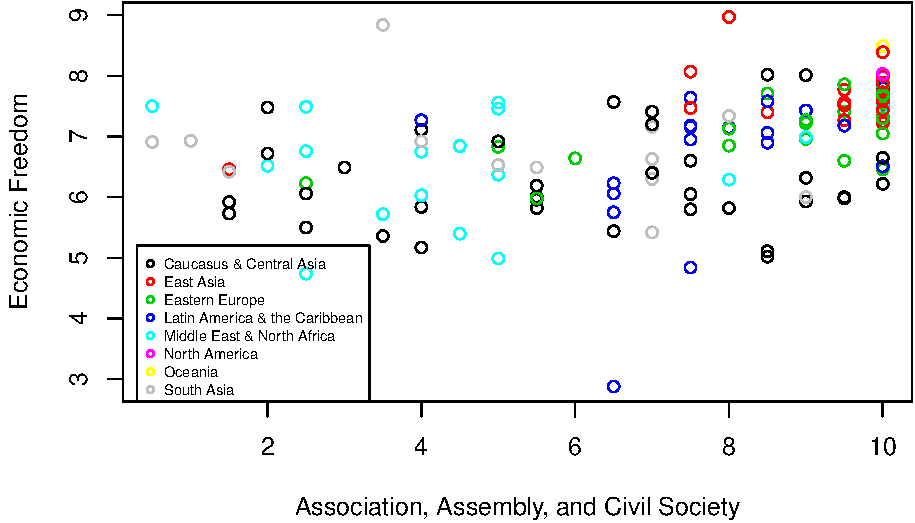
\includegraphics{final_presentation_files/figure-latex/unnamed-chunk-7-1.pdf}

\hypertarget{economic-freedom-vs.expression-and-information}{%
\subsection{Economic Freedom vs.~Expression and
Information}\label{economic-freedom-vs.expression-and-information}}

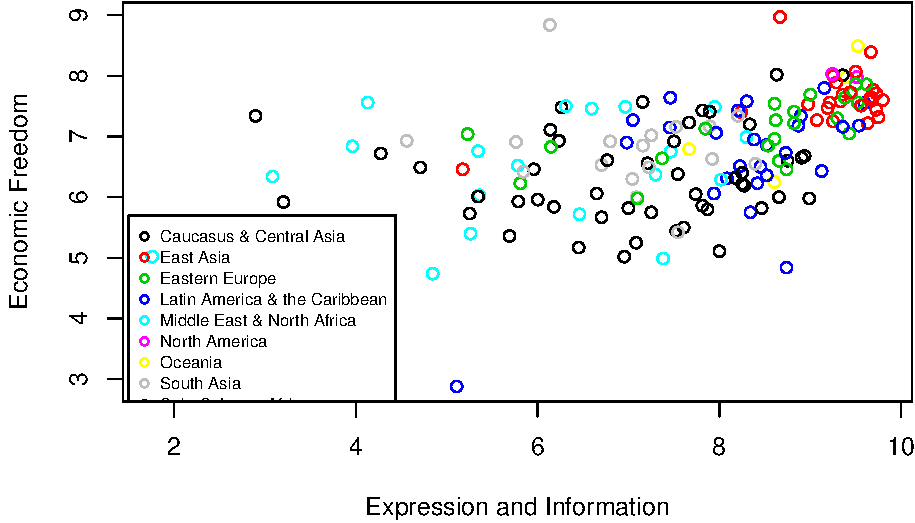
\includegraphics{final_presentation_files/figure-latex/unnamed-chunk-8-1.pdf}

\hypertarget{economic-freedom-vs.identity-and-relationships}{%
\subsection{Economic Freedom vs.~Identity and
Relationships}\label{economic-freedom-vs.identity-and-relationships}}

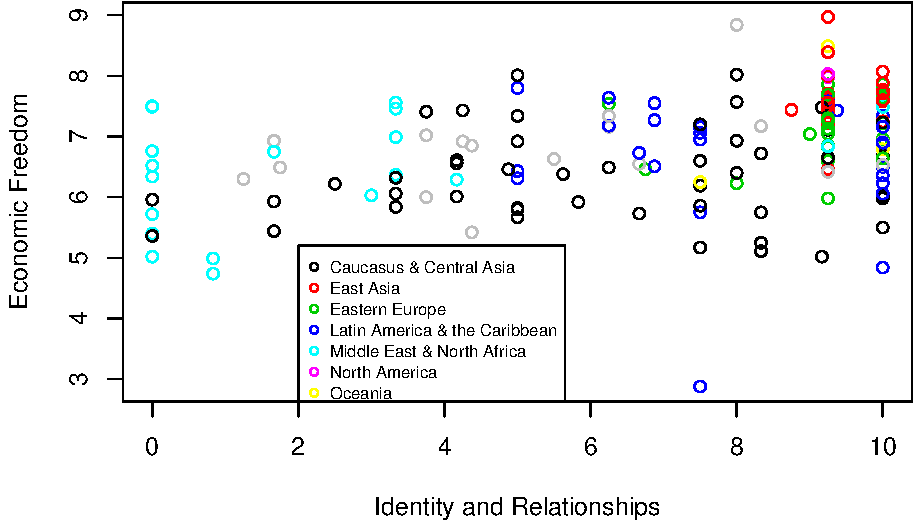
\includegraphics{final_presentation_files/figure-latex/unnamed-chunk-9-1.pdf}

\hypertarget{multiple-regression-of-economic-freedom-and-sub-categories-of-personal-freedom}{%
\subsection{Multiple Regression of Economic Freedom and Sub-Categories
of Personal
Freedom}\label{multiple-regression-of-economic-freedom-and-sub-categories-of-personal-freedom}}

\begin{verbatim}
## 
## Call:
## lm(formula = data$economicfreedom ~ data$rol + data$religion + 
##     data$expression + data$safety + data$relationships + data$movement + 
##     data$assembly)
## 
## Residuals:
##      Min       1Q   Median       3Q      Max 
## -2.82288 -0.34787 -0.01219  0.37809  1.32904 
## 
## Coefficients:
##                     Estimate Std. Error t value Pr(>|t|)    
## (Intercept)         4.039267   0.450908   8.958 3.32e-15 ***
## data$rol            0.301251   0.051946   5.799 4.92e-08 ***
## data$religion      -0.005481   0.046958  -0.117   0.9073    
## data$expression    -0.008769   0.079106  -0.111   0.9119    
## data$safety         0.121946   0.062657   1.946   0.0538 .  
## data$relationships -0.006516   0.023991  -0.272   0.7864    
## data$movement       0.044263   0.029082   1.522   0.1305    
## data$assembly       0.005833   0.039250   0.149   0.8821    
## ---
## Signif. codes:  0 '***' 0.001 '**' 0.01 '*' 0.05 '.' 0.1 ' ' 1
## 
## Residual standard error: 0.6266 on 128 degrees of freedom
##   (26 observations deleted due to missingness)
## Multiple R-squared:  0.5607, Adjusted R-squared:  0.5367 
## F-statistic: 23.34 on 7 and 128 DF,  p-value: < 2.2e-16
\end{verbatim}

\hypertarget{correlation-between-rule-of-law-and-sub-categories-of-personal-freedom}{%
\subsection{Correlation Between Rule of Law and Sub-Categories of
Personal
Freedom}\label{correlation-between-rule-of-law-and-sub-categories-of-personal-freedom}}

\begin{verbatim}
##      [,1]            [,2]                
## [1,] "Gov Size"      "-0.328255694438231"
## [2,] "Legal Systems" "0.90449332414679"  
## [3,] "Money"         "0.522755354935322" 
## [4,] "Trade"         "0.67804130214078"  
## [5,] "Regulation"    "0.685274991389977"
\end{verbatim}

\hypertarget{summary-of-overal-human-freedom-index}{%
\subsection{Summary of Overal Human Freedom
Index}\label{summary-of-overal-human-freedom-index}}

\begin{verbatim}
##    Min. 1st Qu.  Median    Mean 3rd Qu.    Max. 
##   3.766   6.246   6.824   6.890   7.772   8.887
\end{verbatim}

\hypertarget{conclusion}{%
\subsection{Conclusion}\label{conclusion}}

There is a significant relation between economic and personal freedom;
one can be predicted using the other. From the summary of the
regression, we were able to conclude that Rule of Law is the most
signifant in the prediction of economic freedom. Therefore, we examined
the correlation between the rule of law index and the subcategories of
economic freedom.


\end{document}
